If you haven't downloaded and unzipped \href{https://libaoj.in/courses/2021f/MATH3341/zip/Math.3341.zip}{\texttt{Math.3341.zip}}. Download and unzip it under \verb|H:| (H Drive if you are working on the Remote Lab). Change the current working directory by typing \verb|cd H:\Math.3341\Math.3341.Lab.05| in the Command Window, and type \verb|edit lab_05_script| in the Command Window to edit \verb|lab_05_script.m|.

%---------------------------------------------
\section{Formatting Numerical Values}
%---------------------------------------------
\begin{enumerate}[(a)]
    \item Define a variable \verb|x|, of which the value is $e^{\pi}$.
    \item Define a cell array \verb|formatOptions|, of which the entries are listed as follows:
        \begin{enumerate}[(1)]
            \item \verb|rat|
            \item \verb|longeng|
            \item \verb|longg|
            \item \verb|longe|
            \item \verb|long|
            \item \verb|shorteng|
            \item \verb|shortg|
            \item \verb|shorte|
            \item \verb|short|
        \end{enumerate}
    \item Use a for-loop to output \verb|x| in the above formats (do \textsc{not} change the order).
\end{enumerate}
%---------------------------------------------
\section{Formatting Data using \lstinline[style=MATLAB]{fprintf}}
%---------------------------------------------
\begin{enumerate}[(a)]
    \item Define \verb|x| to be column vector ranging from $0$ to $2 \pi$ with $25$ entries, and define \verb|y1|, \verb|y2|, \verb|y3| as follows
        $$
        y_1 = \sin(x/2), \quad
        y_2 = \sin(x), \quad
        y_3 = \sin(2x).
        $$ \item Concatenate column vectors \verb|x|, \verb|y1|, \verb|y2|, \verb|y3|, and store the new 2-D array to \verb|data|.
    \item Print out the heading in the Command Window using \verb|fprintf|, where the heading of the output is \verb|x|, \verb|sin(x/2)|, \verb|sin(x)|, \verb|sin(2x)|, whose widths are $9$. The heading should be left-justified.
    \item Then use a for-loop to loop over each row of \verb|data|: use \verb|fprintf| to print out the numerical values, which have width $9$ with $6$ decimal places, in the Command Window. All numerical values should be left-justified.
\end{enumerate}

%---------------------------------------------
\section{Formatting Data for \LaTeX{}}
%---------------------------------------------
This part we will format \verb|data| (defined above) for \LaTeX{}.
\begin{enumerate}[(a)]
    \item Set the output filename to \verb|sin.tex|, and the permission to \verb|w| (write mode) in \verb|fopen| and store the file handle to the variable \verb|fileHandle|.
    \item Use \verb|fprintf| to print out the setup for \verb|table| and \verb|tabular| environments. The output should be as follows
        \begin{lstlisting}[style=TeX]
\begin{table}[!hbtp]
\centering
\caption{Sine functions}
\label{tab:sin}
\begin{tabular}{lcrr}
\toprule
\midrule
\bottomrule
\end{tabular}
\end{table}
        \end{lstlisting}
    \item Print out the heading of the data, whose column width is $11$ between \verb|\toprule| and \verb|\midrule|. The expected output is as follows:
        \begin{lstlisting}[style=TeX]
        $x$ & $\sin(x/2)$ &   $\sin(x)$ &  $\sin(2x)$ \\
        \end{lstlisting}
    \item Print out the numerical values of each row in \verb|data| between \verb|\midrule| and \verb|\bottomrule| using a for-loop. Each number has width $9$ and $6$ decimal places. Also each number should be enclosed by a pair of \verb|$| and seperated by \verb|&|. The expected output for one of the rows should be as follows
        \begin{lstlisting}[style=TeX]
$ 0.000000$ & $ 0.000000$ & $ 0.000000$ & $ 0.000000$ \\
        \end{lstlisting}
    \item Print the content of \verb|sin.tex| by calling \verb|type('sin.tex')|.
\end{enumerate}
%---------------------------------------------
\section{Plotting Multiple Functions using for-loop}
%---------------------------------------------
\begin{enumerate}[(a)]
    \item Define a cell array \verb|styles|. The elements are plotting styles, i.e.,
        \begin{enumerate}[(1)]
            \item solid line with circle as the marker;
            \item dashdot line with diamond as the marker;
            \item dashed line with triangle (up) as the marker.
        \end{enumerate}
    \item Define another cell array \verb|y|, of which the entries are \verb|y1|, \verb|y2|, and \verb|y3|.
    \item Then use a for-loop to plot each entries of \verb|y| versus \verb|x| with in the same figure window the above styles (in the same order).
    \item Set legend, labels, grid, and title. Change the range of $x$-axis to $[0, 2\pi]$, and that of $y$-axis to $[-1, 1]$. Set the following properties as you did in last lab. The expected result is shown in Figure \ref{fig:sin}.
    \begin{itemize}
        \item \verb|XTick| to \verb|[0, pi / 2, pi, 3 * pi / 2, 2 * pi]|;
        \item \verb|XTickLabel| to \verb|{'0', '$\pi/2$', '$\pi$', '$3 \pi/2$', '$2\pi$'}|;
        \item \verb|GridLineStyle| to \verb|'--'|;
        \item \verb|Box| to \verb|'on'|;
        \item \verb|BoxStyle| to \verb|'full'|.
    \end{itemize}
    \item Then save the plot using the following lines of commands:
        \begin{lstlisting}[style=MATLAB]
name = 'lab_05_plot';
fig = figure(1);                         % Set figure i as current figure window
set(fig, 'PaperPositionMode', 'auto');   % Set paper position mode to 'auto'
pos = get(fig, 'PaperPosition');         % Get figure window paper position
set(fig, 'PaperSize', [pos(3) pos(4)]);  % Set figure paper size
print(fig, '-dpdf', name);               % Save figure
        \end{lstlisting}
\end{enumerate}
%---------------------------------------------
Type \verb|diary('lab_05_output.txt')| in the Command Window, run the script file \verb|lab_05_script.m|, and type \verb|diary off| in the Command Window. Upload \verb|lab_05_output.txt|, \verb|sin.tex|, and \verb|lab_05_script.m| to the folder \verb|src| on Overleaf.

On Overleaf, open \verb|body.tex| under the folder \verb|LaTeX|. In the last section of the report, you will reproduce Section \ref{sec:bol} using \LaTeX{}. You may find the following helpful:

\begin{itemize}
    \item You may use enviroments such as  \verb|align|, \verb|figure|, and \verb|table|.
    \item You may use \verb|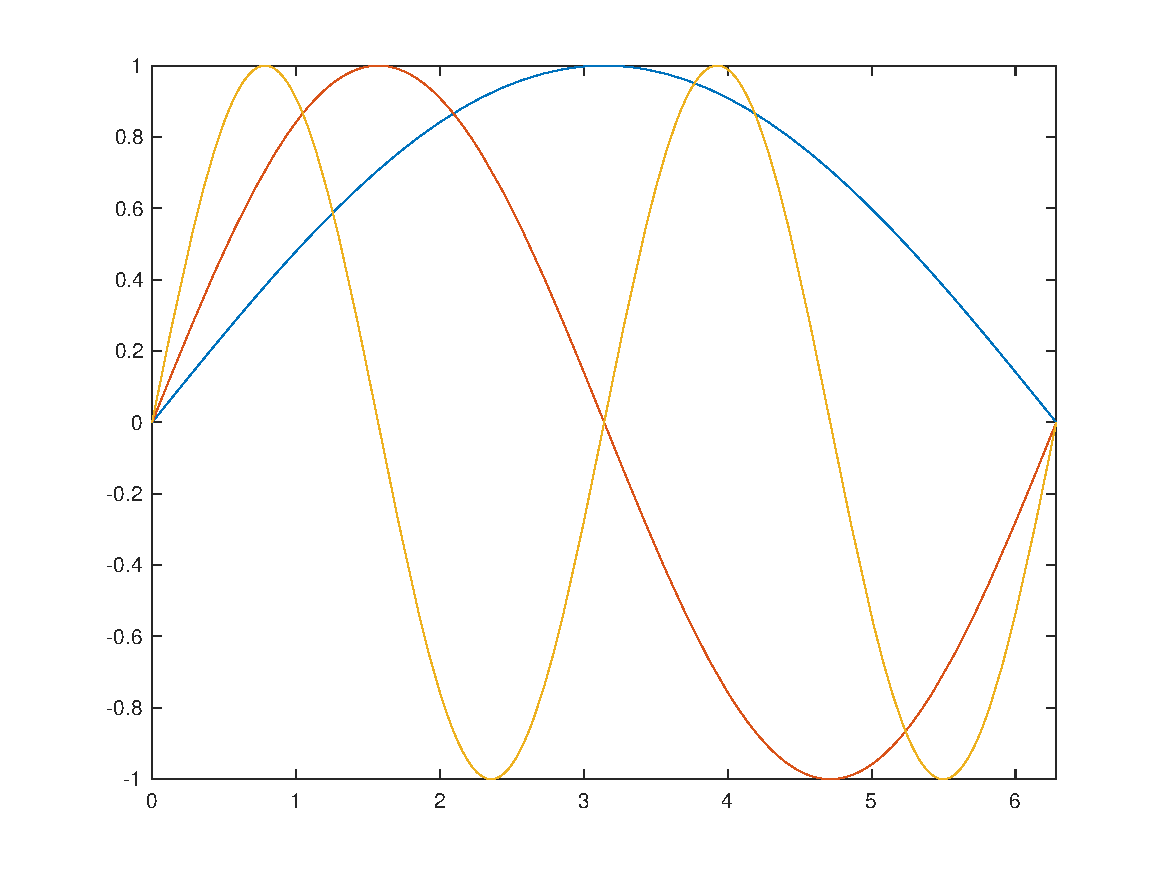
\includegraphics[width=amount unit]{/path/to/figure.pdf}| to specify the width of a figure. In our case, the width of the figure is \verb|0.75\textwidth|.
    \item For special characters, you may look them up in \href{https://libaoj.in/files/LaTeX.Mathematical.Symbols.pdf}{\LaTeX{}.Mathematics.Symbols.pdf}.
    \item You may use \verb|\begin{table}[!hbtp]
\centering
\caption{Sine functions}
\label{tab:sine}
\begin{tabular}{lcrr}
\toprule
        $x$ & $\sin(x/2)$ &   $\sin(x)$ &  $\sin(2x)$ \\
\midrule
$ 0.000000$ & $ 0.000000$ & $ 0.000000$ & $ 0.000000$ \\
$ 0.261799$ & $ 0.130526$ & $ 0.258819$ & $ 0.500000$ \\
$ 0.523599$ & $ 0.258819$ & $ 0.500000$ & $ 0.866025$ \\
$ 0.785398$ & $ 0.382683$ & $ 0.707107$ & $ 1.000000$ \\
$ 1.047198$ & $ 0.500000$ & $ 0.866025$ & $ 0.866025$ \\
$ 1.308997$ & $ 0.608761$ & $ 0.965926$ & $ 0.500000$ \\
$ 1.570796$ & $ 0.707107$ & $ 1.000000$ & $ 0.000000$ \\
$ 1.832596$ & $ 0.793353$ & $ 0.965926$ & $-0.500000$ \\
$ 2.094395$ & $ 0.866025$ & $ 0.866025$ & $-0.866025$ \\
$ 2.356194$ & $ 0.923880$ & $ 0.707107$ & $-1.000000$ \\
$ 2.617994$ & $ 0.965926$ & $ 0.500000$ & $-0.866025$ \\
$ 2.879793$ & $ 0.991445$ & $ 0.258819$ & $-0.500000$ \\
$ 3.141593$ & $ 1.000000$ & $ 0.000000$ & $-0.000000$ \\
$ 3.403392$ & $ 0.991445$ & $-0.258819$ & $ 0.500000$ \\
$ 3.665191$ & $ 0.965926$ & $-0.500000$ & $ 0.866025$ \\
$ 3.926991$ & $ 0.923880$ & $-0.707107$ & $ 1.000000$ \\
$ 4.188790$ & $ 0.866025$ & $-0.866025$ & $ 0.866025$ \\
$ 4.450590$ & $ 0.793353$ & $-0.965926$ & $ 0.500000$ \\
$ 4.712389$ & $ 0.707107$ & $-1.000000$ & $ 0.000000$ \\
$ 4.974188$ & $ 0.608761$ & $-0.965926$ & $-0.500000$ \\
$ 5.235988$ & $ 0.500000$ & $-0.866025$ & $-0.866025$ \\
$ 5.497787$ & $ 0.382683$ & $-0.707107$ & $-1.000000$ \\
$ 5.759587$ & $ 0.258819$ & $-0.500000$ & $-0.866025$ \\
$ 6.021386$ & $ 0.130526$ & $-0.258819$ & $-0.500000$ \\
$ 6.283185$ & $ 0.000000$ & $-0.000000$ & $-0.000000$ \\
\bottomrule
\end{tabular}
\end{table}
| to include the table you got from MATLAB.
\end{itemize}

Recompile and submit the PDF file generated by Overleaf to WyoCourses.
%---------------------------------------------

\newpage
\section{Basics of \LaTeX{}}
\label{sec:bol}
\subsection{Sine functions}
For given $x \in [0, 2\pi]$ with step size $\pi/12$, we can obtain the evaluations of \eqref{eq:y1}, \eqref{eq:y2}, \eqref{eq:y3} at $x$ (see Table \ref{tab:sin}), and the corresponding plot (see Figure \ref{fig:sin}).
\begin{align}
y_1 & = \sin(x/2) \label{eq:y1} \\
y_2 & = \sin(x)   \label{eq:y2} \\
y_3 & = \sin(2x)  \label{eq:y3}
\end{align}
\begin{table}[!hbtp]
\centering
\caption{Sine functions}
\label{tab:sine}
\begin{tabular}{lcrr}
\toprule
        $x$ & $\sin(x/2)$ &   $\sin(x)$ &  $\sin(2x)$ \\
\midrule
$ 0.000000$ & $ 0.000000$ & $ 0.000000$ & $ 0.000000$ \\
$ 0.261799$ & $ 0.130526$ & $ 0.258819$ & $ 0.500000$ \\
$ 0.523599$ & $ 0.258819$ & $ 0.500000$ & $ 0.866025$ \\
$ 0.785398$ & $ 0.382683$ & $ 0.707107$ & $ 1.000000$ \\
$ 1.047198$ & $ 0.500000$ & $ 0.866025$ & $ 0.866025$ \\
$ 1.308997$ & $ 0.608761$ & $ 0.965926$ & $ 0.500000$ \\
$ 1.570796$ & $ 0.707107$ & $ 1.000000$ & $ 0.000000$ \\
$ 1.832596$ & $ 0.793353$ & $ 0.965926$ & $-0.500000$ \\
$ 2.094395$ & $ 0.866025$ & $ 0.866025$ & $-0.866025$ \\
$ 2.356194$ & $ 0.923880$ & $ 0.707107$ & $-1.000000$ \\
$ 2.617994$ & $ 0.965926$ & $ 0.500000$ & $-0.866025$ \\
$ 2.879793$ & $ 0.991445$ & $ 0.258819$ & $-0.500000$ \\
$ 3.141593$ & $ 1.000000$ & $ 0.000000$ & $-0.000000$ \\
$ 3.403392$ & $ 0.991445$ & $-0.258819$ & $ 0.500000$ \\
$ 3.665191$ & $ 0.965926$ & $-0.500000$ & $ 0.866025$ \\
$ 3.926991$ & $ 0.923880$ & $-0.707107$ & $ 1.000000$ \\
$ 4.188790$ & $ 0.866025$ & $-0.866025$ & $ 0.866025$ \\
$ 4.450590$ & $ 0.793353$ & $-0.965926$ & $ 0.500000$ \\
$ 4.712389$ & $ 0.707107$ & $-1.000000$ & $ 0.000000$ \\
$ 4.974188$ & $ 0.608761$ & $-0.965926$ & $-0.500000$ \\
$ 5.235988$ & $ 0.500000$ & $-0.866025$ & $-0.866025$ \\
$ 5.497787$ & $ 0.382683$ & $-0.707107$ & $-1.000000$ \\
$ 5.759587$ & $ 0.258819$ & $-0.500000$ & $-0.866025$ \\
$ 6.021386$ & $ 0.130526$ & $-0.258819$ & $-0.500000$ \\
$ 6.283185$ & $ 0.000000$ & $-0.000000$ & $-0.000000$ \\
\bottomrule
\end{tabular}
\end{table}

\begin{figure}[!hbtp]
    \centering
    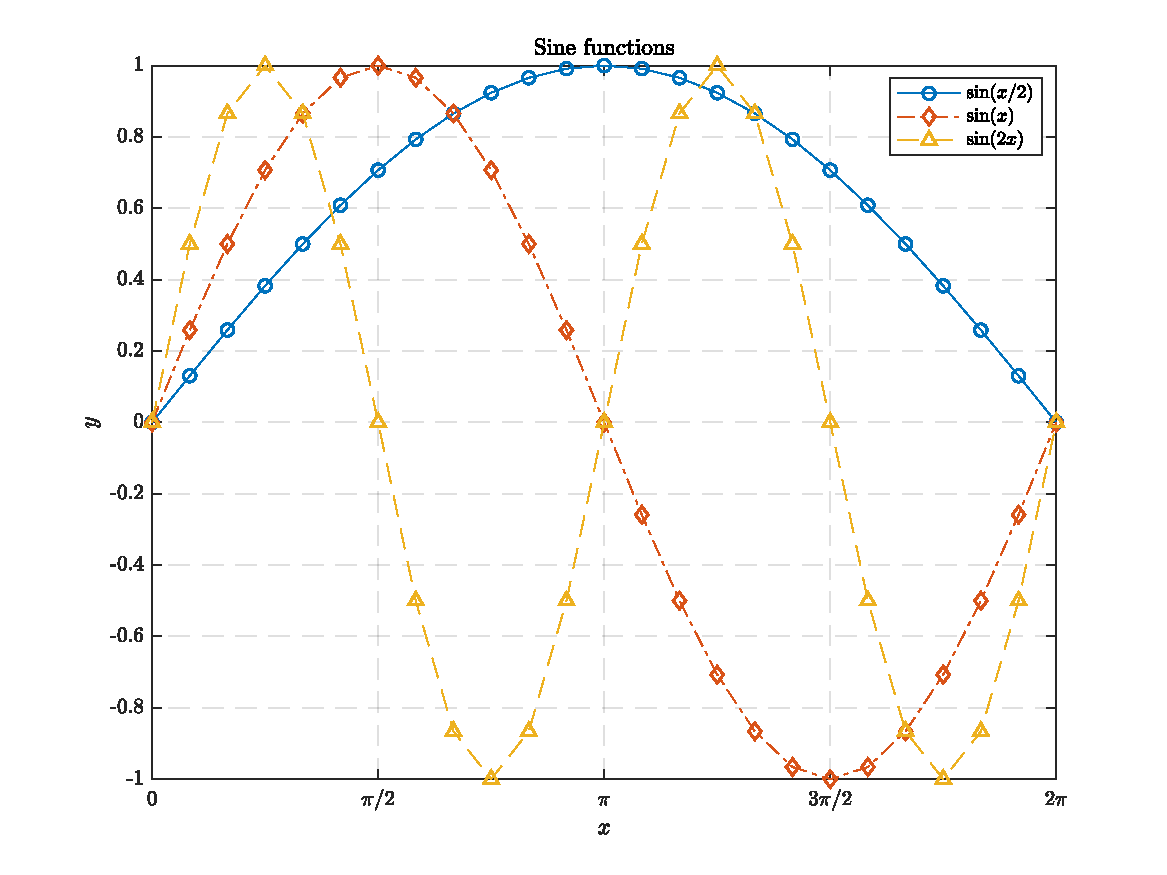
\includegraphics[width=0.75\textwidth]{../Math.3341.Lab.05.ans/lab_05_plot.pdf}
    \caption{Sine functions}
    \label{fig:sin}
\end{figure}
